%!TEX root = ../dokumentation.tex

\chapter{Grundlagen der Arbeit}

Im folgenden werden nun die Gr
%title wird unter dem Bsp. abgedruckt
%caption wird im Verzeichnis abgedruckt
%label wird zum referenzieren benutzt, muss einzigartig sein.

\section{Raspberry Pi 3 Model B}
Ein \textit{Raspberry Pi} ist ein Kreditkarten großer Computer welcher an einen Computerbildschirm oder einem Fernseher angeschlossen wird und mit einer Standardtastatur und -maus verwendet werden kann. Im Vergleich zu einem normalen Desktop Computer stellt der Raspberry Pi mit einem Preis rund 30 Euro eine sehr günstige Alternative dar. Der Raspberry Pi wurde entwickelt um Personen in jedem Alter die Möglichkeit zu bieten einen Computer zu benutzen und programmieren zu lernen. Das Standard Betriebssystem des Raspberry Pi basiert auf einer eigen entwickelten Linux Distribution von Raspberry Pi mit dem Namen \textit{Raspbian}. \autocite{what_is_a_raspberry_pi?_2019}
\begin{figure}[h]
	\centering
	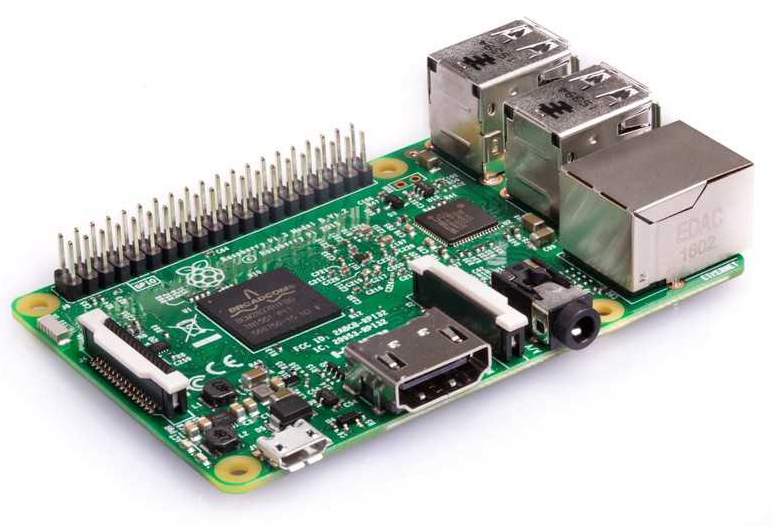
\includegraphics[scale=0.35]{Raspberry_Pi_3_Model_B.jpg}
	\caption{Beispielbild - Raspberry Pi 3 Model B \autocite{raspberry_pi_2019}}
	\label{img:grafik-RaspberryPi3}
\end{figure}
\newline

Auf den in der Abbildung \ref{img:grafik-RaspberryPi3} dargestellten Raspberry Pi handelt es sich um ein Gerät der neusten Generationen, den Raspberry Pi 3 Model B. Er zeichnet sich durch eine neue 64-Bit \ac{ARM}-\ac{CPU} mit 1.2 \ac{GHz} aus und besitzt dazu 1 \ac{GB} \ac{RAM}. Des Weiteren stellt er sämtliche Anschlüsse wie z.B. 4 \ac{USB} Ports, RJ45 Anschluss, \ac{HDMI} Anschluss sowie 40 \ac{GPIO} Ports zur Verfügung. Mit dem neusten Model des Raspberry Pi wurde zudem noch eine \ac{WLAN} sowie Bluetooth Karte integriert. In der Kombination mit dem \ac{SD-Karten} Slot, welcher als Speicher benutzt wird, stellt der Raspberry Pi einen vollwertigen Computer dar. \autocite{kurniawan_2016}
 
\section{Go}
\textit{Go} oftmals auch \textit{Golang} genannt ist eine von \textit{Google Inc.} entwickelte typsichere, kompakte und effiziente, kompilierbare Programmiersprache, die als Open-Source Projekt seit 2009 initial von Robert Griesemer, Rob Pike, and Ken Thompson entwickelt wird \autocite{documentation_the_go_programming_language_2019}. Grob gesagt reiht sich Go zwischen C/C++ und Perl ein. Google legt einen großen Wert darauf, Go als Sprache für die Systemprogrammierung zu positionieren, setzt dazu aber nicht typische Mittel wie einen Garbage Collector sowie die Unterstützung zur Parallel und Multicore Verarbeitung ein \autocite{feike_blass_2012}. Go überzeugt vor allen Dingen durch seine Einfachheit beim Programmieren sowie durch die Geschwindigkeit beim kompilieren und ausführen des Codes. Zusätzlich wird die Nebenläufigkeit von Prozessen unterstützt, die \textit{Goroutinen} genannt werden und über Kanäle miteinander kommunizieren können. \autocite{donovan_kernighan_2016}


\section{Git and GitHub}
\textit{Git} ist eines der bekanntesten Versionskontrollsysteme welches 2005 von Linus Torvalds entwickelt wurde. Unter einem Versionskontrollsystem wird ein Software verstanden, die die Veränderung von Dateien über einen Zeitraum aufzeichnet und speichert. Dadurch wird es auch ermöglicht zu jedem Zeitpunkt wieder auf einen alten Dateizustand zurückzuspringen.
Genauer genommen ist \textit{Git} ein verteiltest Versionskontrollsystem, was bedeutet dass alle Personen in einem  Projekt nicht nur den aktuellen Stand sondern auch die komplette Historie einsehen können. \autocite{preissel_stachmann_2017}
\newline
\newline
\textit{GitHub} ist eine Webseite in der man eine Kopie eines \textit{Git} Repository speichern kann. Dadurch ergibt sich ein zentralisierter Ort um einfach mit anderen Personen an einem Projekt  arbeiten zu können. \textit{GitHub} bietet vor allen Dingen durch seine weiteren Funktionen wie z.B. ein Web Interface, ein Wiki sowie einen Bereich zum diskutieren und bewerten von Änderungen, eine ausgewogene Arbeitsumgebung zum Entwickeln von Software. \autocite{bell_2014}